\documentclass[a4paper,12pt]{book}
\usepackage[english]{babel}
\usepackage[a4paper, inner=2cm, outer=3cm, top=3cm, bottom=3cm, bindingoffset=0.5cm]{geometry}
\usepackage{minitoc}


\usepackage{graphicx}
\usepackage{eso-pic}
\usepackage{xcolor}
\usepackage{xcolor-material}
\usepackage{tikz}
\usepackage{hyperref}
\hypersetup{ % it doesn't work near toc, has to be global in here.
    colorlinks=true,
    linkcolor=MaterialPink700,
    urlcolor=MaterialPink700,
    filecolor=MaterialGreen,
    pdfborder={0 0 0},
}

\RequirePackage{fancyhdr}
\RequirePackage{lastpage}
\pagestyle{fancy} % these 3 lines set the footer to the middle with total page #.

% fancier chapter title
\usepackage[]{titlesec}%

\usepackage{blindtext}

\definecolor{bannercolor}{rgb}{0.3922,0.5843,0.9294}

\linespread{1.2} % make lines less crowded

% headers
\fancyhf{}
\fancyhead[LO]{\nouppercase{\rightmark}}
\fancyhead[RE]{\nouppercase{\leftmark}}
\fancyhead[LE,RO]{\thepage}

\begin{document}
%----------------------------------------------------------------------------------------
%	TITLE PAGE
%----------------------------------------------------------------------------------------
    \title{Clustering the interstellar medium}

    \begingroup
    \thispagestyle{empty}
	\AddToShipoutPicture*{\put(0,0){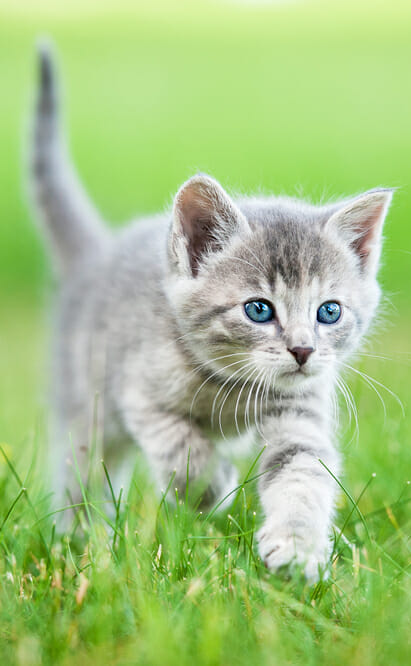
\includegraphics[scale=3]{cat1}}} % Image background

    \vspace*{3.75cm}
	\hspace*{-4cm}
	%\put(0 mm, 142 mm) % copied from https://www.overleaf.com/latex/templates/matnat-compendium/xbfgbfgzpcxz
	%{ % Given a picture, we overlay a banner, rather than modifying the picture itself
		
\begin{tikzpicture}[scale = 1mm]
			%\filldraw[white, opacity = 0.8]
			%(0, 2.5) rectangle (\paperwidth, 3.73);
			%\filldraw[white, opacity = 0.6]
			%(0, 0) rectangle (\paperwidth, 2.5);
			\filldraw[bannercolor, opacity = 0.3]
			(0, 0) rectangle (\paperwidth, 3.5);
		\end{tikzpicture}
	%}
	\centering
	\vspace*{-9cm}
	\par\normalfont\fontsize{35}{35}\sffamily\selectfont
	\textbf{Do Cats Always Land on Their Feet?}\\
	{\LARGE That's how they have 9 lives!}\par % Book title
	\vspace*{1cm}
	{\Huge Flying Cats}\par % Author name
    \endgroup

%----------------------------------------------------------------------------------------
%	COPYRIGHT PAGE
%----------------------------------------------------------------------------------------
    \newpage
    \thispagestyle{empty}
    ~\vfill

    \noindent Copyright \copyright\ 2021 John Smith\\ % Copyright notice

    \noindent \textsc{Published by Publisher}\\ % Publisher

    \noindent \textsc{book-website.com}\\ % URL

    \noindent Licensed under the Creative Commons Attribution-NonCommercial 3.0 Unported License
    (the ``License'').
    You may not use this file except in compliance with the License.
    You may obtain a copy of the License at \url{https://creativecommons.org/licenses/by-nc/3.0}.
    Unless required by applicable law or agreed to in writing, software distributed under the
    License is distributed on an \textsc{``as is'' basis, without warranties or conditions of any
    kind}, either express or implied.
    See the License for the specific language governing permissions and limitations under the
    License.\\ % License information, replace this with your own license (if any)

    \noindent \textit{First printing, March 2021} % Printing/edition date

%----------------------------------------------------------------------------------------
%	TABLE OF CONTENTS
%----------------------------------------------------------------------------------------
    \pagestyle{empty} % Disable headers and footers for the following pages

    % https://texblog.org/2008/09/15/create-small-tocslofslots-using-minitoc/
    \dominitoc % mini toc for chapters
    \mtcsetrules{*}{off} % remove top/bottom lines around minitoc
    \tableofcontents % Print the table of contents itself

    % Forces the first chapter to start on an odd page so it's on the right side of the book
    %\cleardoublepage


%----------------------------------------------------------------------------------------
%	Chapters
%----------------------------------------------------------------------------------------
    \pagestyle{fancy} % Enable headers and footers again

    
\chapter{Introduction}
\minitoc

This is an introduction.

\section{Environment Setup}

This is a husky.

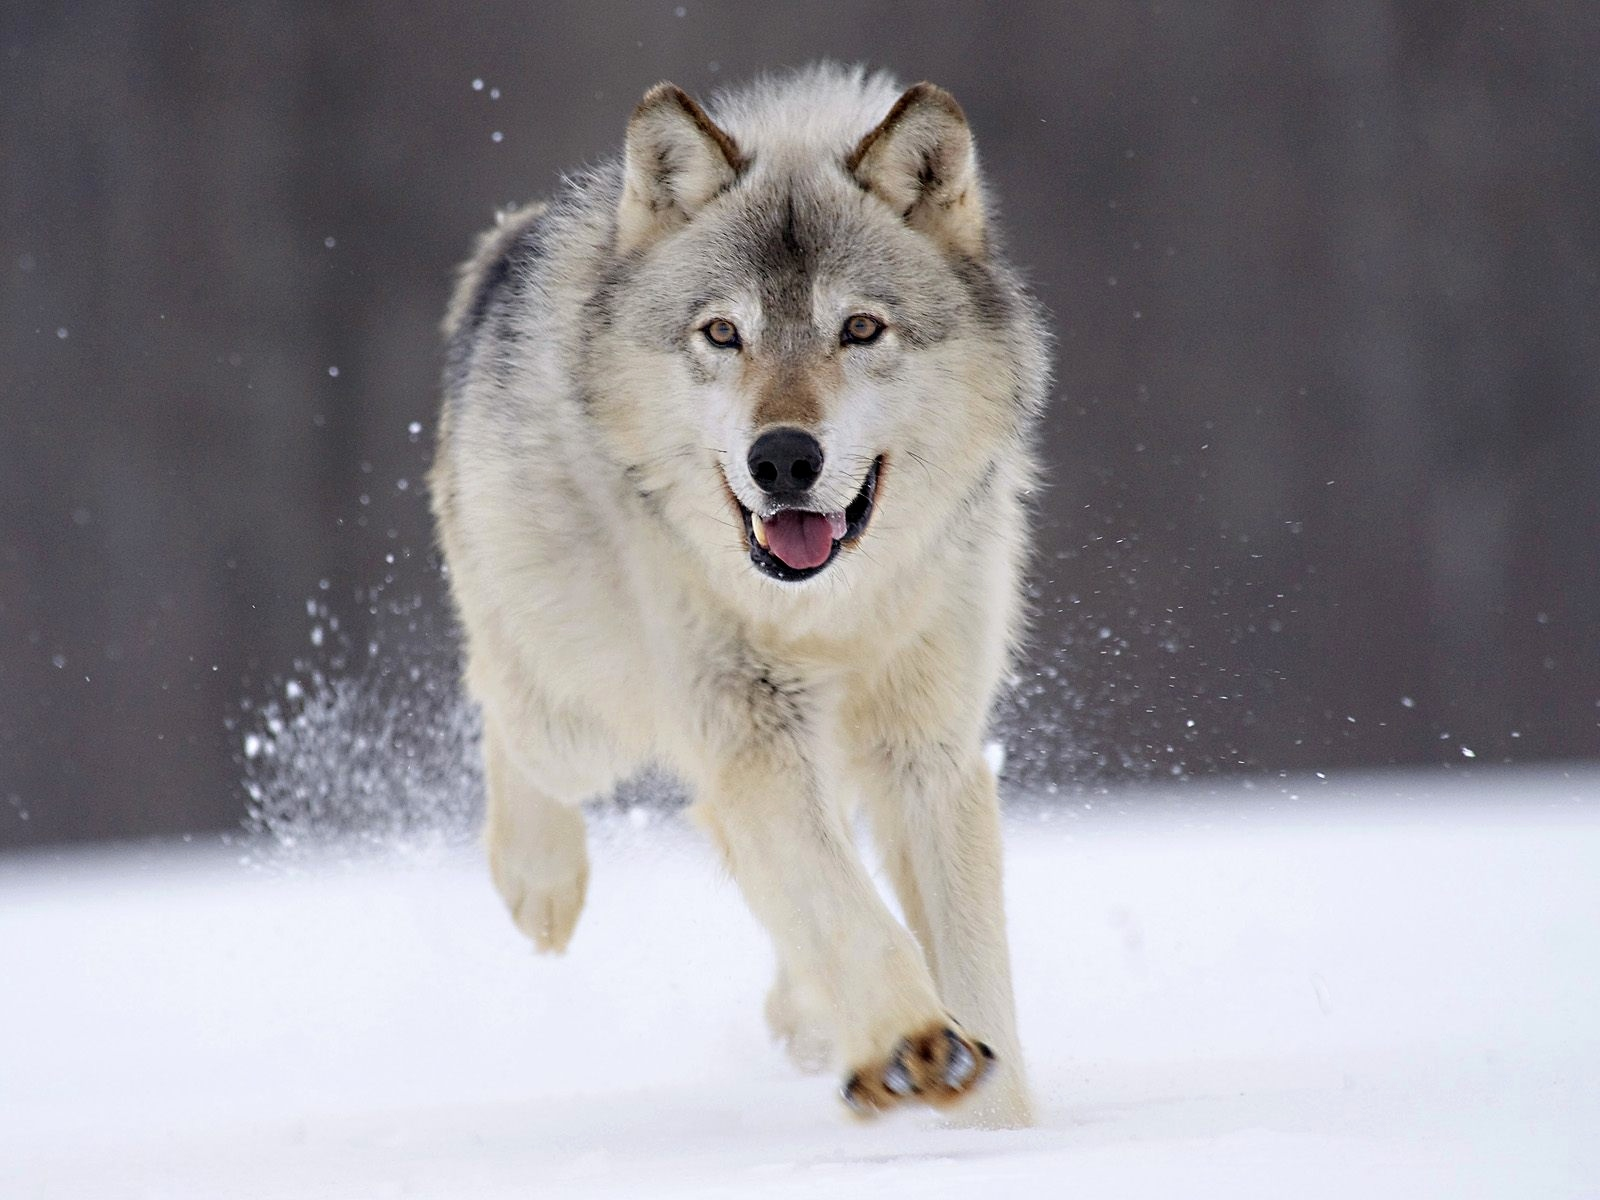
\includegraphics[scale=0.25]{chapter1/husky}

\blindtext[3]

\section{Get work done}

\blindtext[3]


    

\chapter{Deep Dive}
\minitoc

It's time to get more detailed facts.

\section{Environment Setup}

This is a treasure, 汗血宝马.

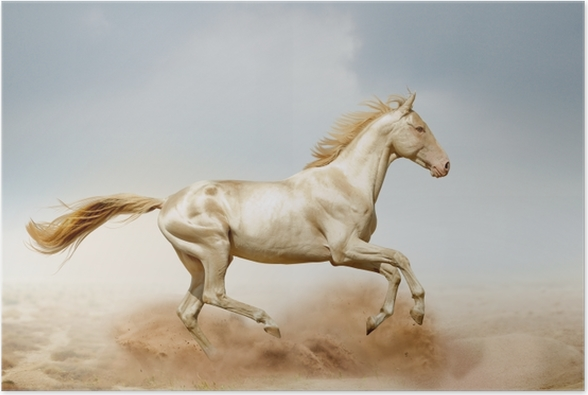
\includegraphics[scale=3]{chapter2/akhal_teke_horse}

\blindtext[3]

\section{Get work done}

\blindtext[3]

\section{Get work done}

\blindtext[3]

\end{document}
